\chapter{Resultados}

Uno de los principales problemas que motivaron el método de optimización propuesto en este escrito es la dificultad de diversas arquitecturas de aprendizaje profundo para capturar propiedades topológicas globales en estructuras tridimensionales, especialmente en superficies de género mayor que uno. Aunque modelos basados en operadores neuronales, mecanismos de atención o nubes de puntos han mostrado buenos resultados en tareas geométricas, su desempeño puede verse limitado cuando la clasificación depende de invariantes topológicos como la característica de Euler o el género, ya que suelen dar prioridad a información local o relaciones geométricas extrínsecas sin incorporar explícitamente la conectividad de los puntos que conforman la malla.
En este contexto surge EuLearn \cite{2025eulearn}, una base de datos diseñada para evaluar modelos de aprendizaje profundo en tareas de clasificación topológica. A diferencia de otros conjuntos de datos tridimensionales enfocados en reconocimiento de objetos, EuLearn contiene superficies con géneros controlados, lo que permite analizar si una arquitectura es capaz de distinguir entre diferentes clases topológicas a partir de campos escalares, nubes de puntos, mallas trianguladas o gráficas asociadas.
Uno de los principales retos al trabajar con estas superficies es el tamaño y la complejidad de las mallas, compuestas por una gran cantidad de vértices, aristas y caras. Esto incrementa el costo computacional y dificulta el entrenamiento eficiente de los modelos. Además, una reducción aleatoria de puntos puede eliminar relaciones de adyacencia relevantes para la clasificación topológica. Por ello, en esta tesis se analiza un método de optimización sobre gráficas que reduce la representación original de la malla preservando relaciones estructurales esenciales.
El método propuesto puede interpretarse como una estrategia de muestreo estructurado sobre la gráfica asociada a la malla. A diferencia de enfoques basados únicamente en distancia euclidiana, como ocurre en ciertas etapas de arquitecturas tipo PointNet++, esta aproximación considera la conectividad intrínseca de la superficie. De esta manera, se reduce la dimensionalidad de los datos de entrada sin descartar información local relevante, facilitando el entrenamiento y favoreciendo una mejor capacidad de generalización.
A lo largo de este capítulo se presentan las arquitecturas utilizadas para evaluar el método propuesto, incluyendo Fourier Neural Operator, Dynamic Graph CNN, PointNet, PointNet++, modelos basados en atención, Graph Sampled PointNet y Graph Sampled Attention. Asimismo, se comparan los resultados obtenidos sobre EuLearn y se discute cómo el uso de información de adyacencia mejora el aprendizaje de propiedades topológicas globales asociadas al género y a la característica de Euler de superficies tridimensionales.

\section{Arquitecturas utilizadas}
A lo largo de la evaluación de las superficies contenidas en la base de datos \cite{2025eulearn}, se utilizan diversas arquitecturas de aprendizaje profundo, cada una con características particulares que las hacen adecuadas para procesar datos tridimensionales. A continuación, se describen brevemente las principales arquitecturas empleadas.

\subsection{Fourier Neural Operator}
El modelo Fourier Neural Operator (FNO) es una arquitectura diseñada para aprender operadores entre espacios de funciones. En el contexto de EuLearn, esta arquitectura se utiliza sobre la representación continua de la superficie, en lugar de operar directamente sobre la nube de puntos o la malla triangular. Su idea principal consiste primero en transformar información geométrica en un conjunto de frecuencias mediante la transformada de Fourier, posteriormente la red aprende qué patrones de esas frecuencias son relevantes y, finalmente transforma nuevamente la información al espacio original mediante la transformada inversa de Fourier. De esta forma esta estrategia permite capturar relaciones globales en la superficie lo cual es de suma importancia para la clasificacón topológica.

\begin{figure}[H]
    \centering
    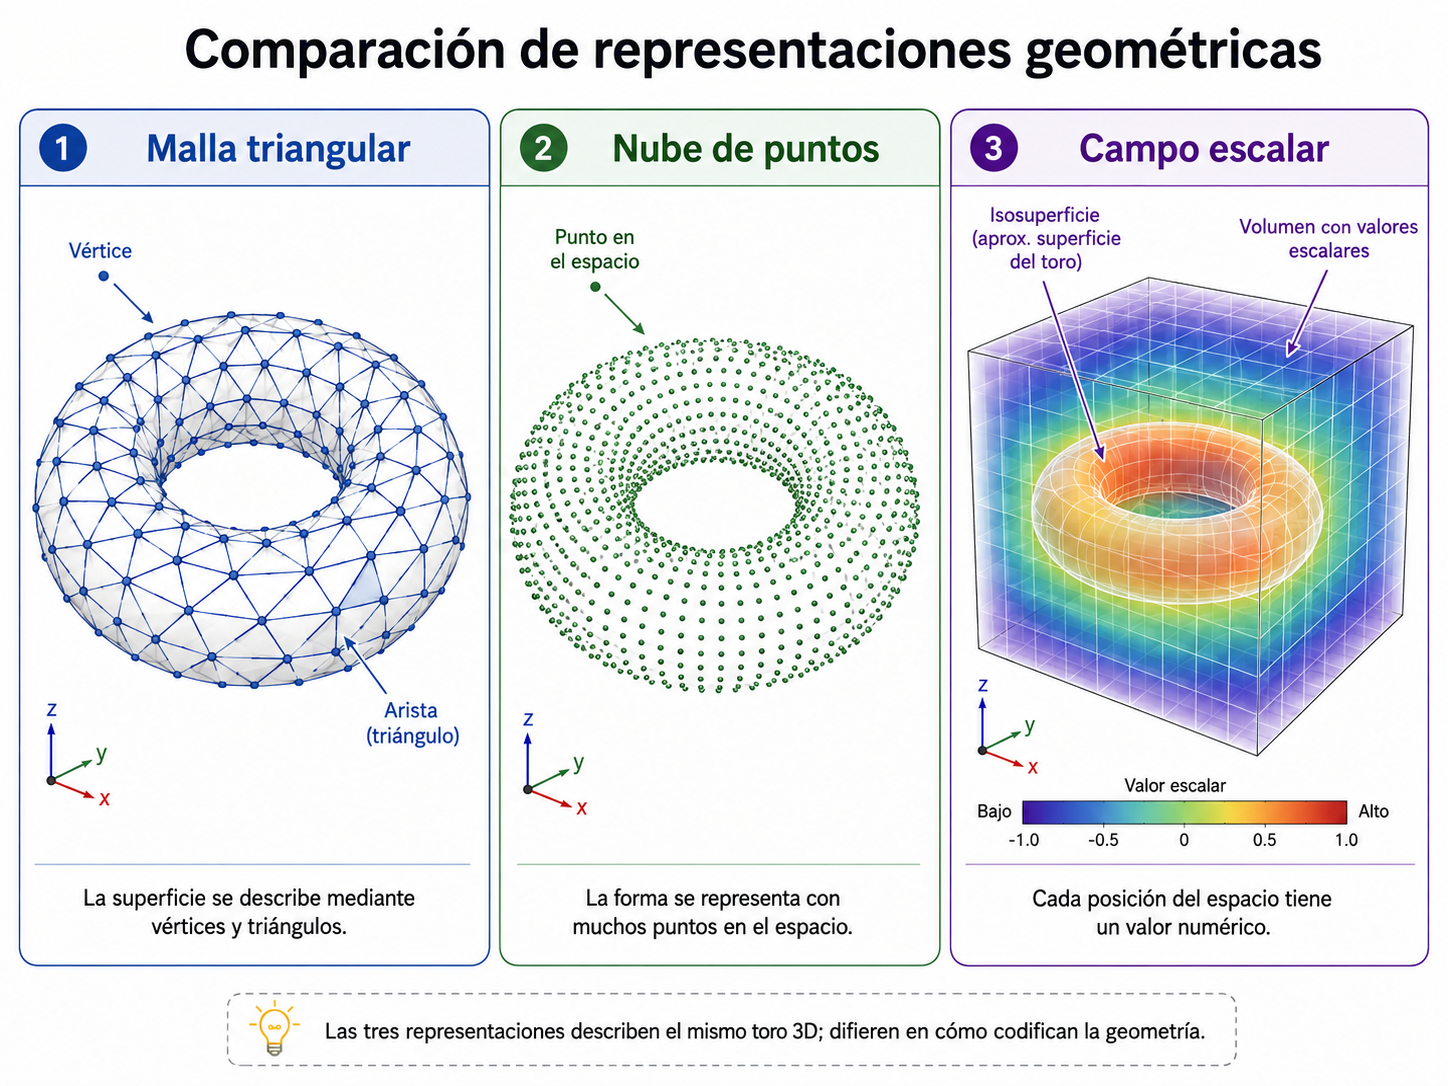
\includegraphics[width=\textwidth]{img/comparacion.png}
    \caption{Comparación entre malla triangulada, nube de puntos y campo escalar.}
    \label{fig:comparacion}
\end{figure}

De manera general, un bloque FNO puede escribirse como
\[
\sigma
\left(
Wv_t(x)
+
\mathcal{F}^{-1}
\left(
R_\theta \cdot \mathcal{F}(v_t)
\right)(x)
\right),
\]
donde $(v_t)$ es la representación de entrada en la capa $(t)$, $(W)$ es una transformación lineal local, $(\mathcal{F})$ y $(\mathcal{F}^{-1})$ denotan la transformada de Fourier y su inversa, respectivamente, $(R_\theta)$ es un tensor de pesos aprendibles en el dominio frecuencial y $(\sigma)$ es una función de activación.

\subsection{Dynamic Graph CNN}
La arquitectura Dynamic Graph CNN (DGCNN) es una arquitectura diseñada para procesar nubes de puntos mediante convoluciones definidas sobre gráficas dinámicas. Para cada punto , identifica los más cercanos, usualmente mediante (k)-nearest neighbors, y los conecta formando una gráfica, de esta forma, la red analiza la relación entre cada punto y sus vecinos para aprender características locales de la forma de la superficie. Además, estas conexiones pueden volver a calcularse durante las diferentes capas de la red, por lo que la gráfica cambia dinámicamente conforme el modelo aprende nuevas características.

\begin{figure}[H]
    \centering
    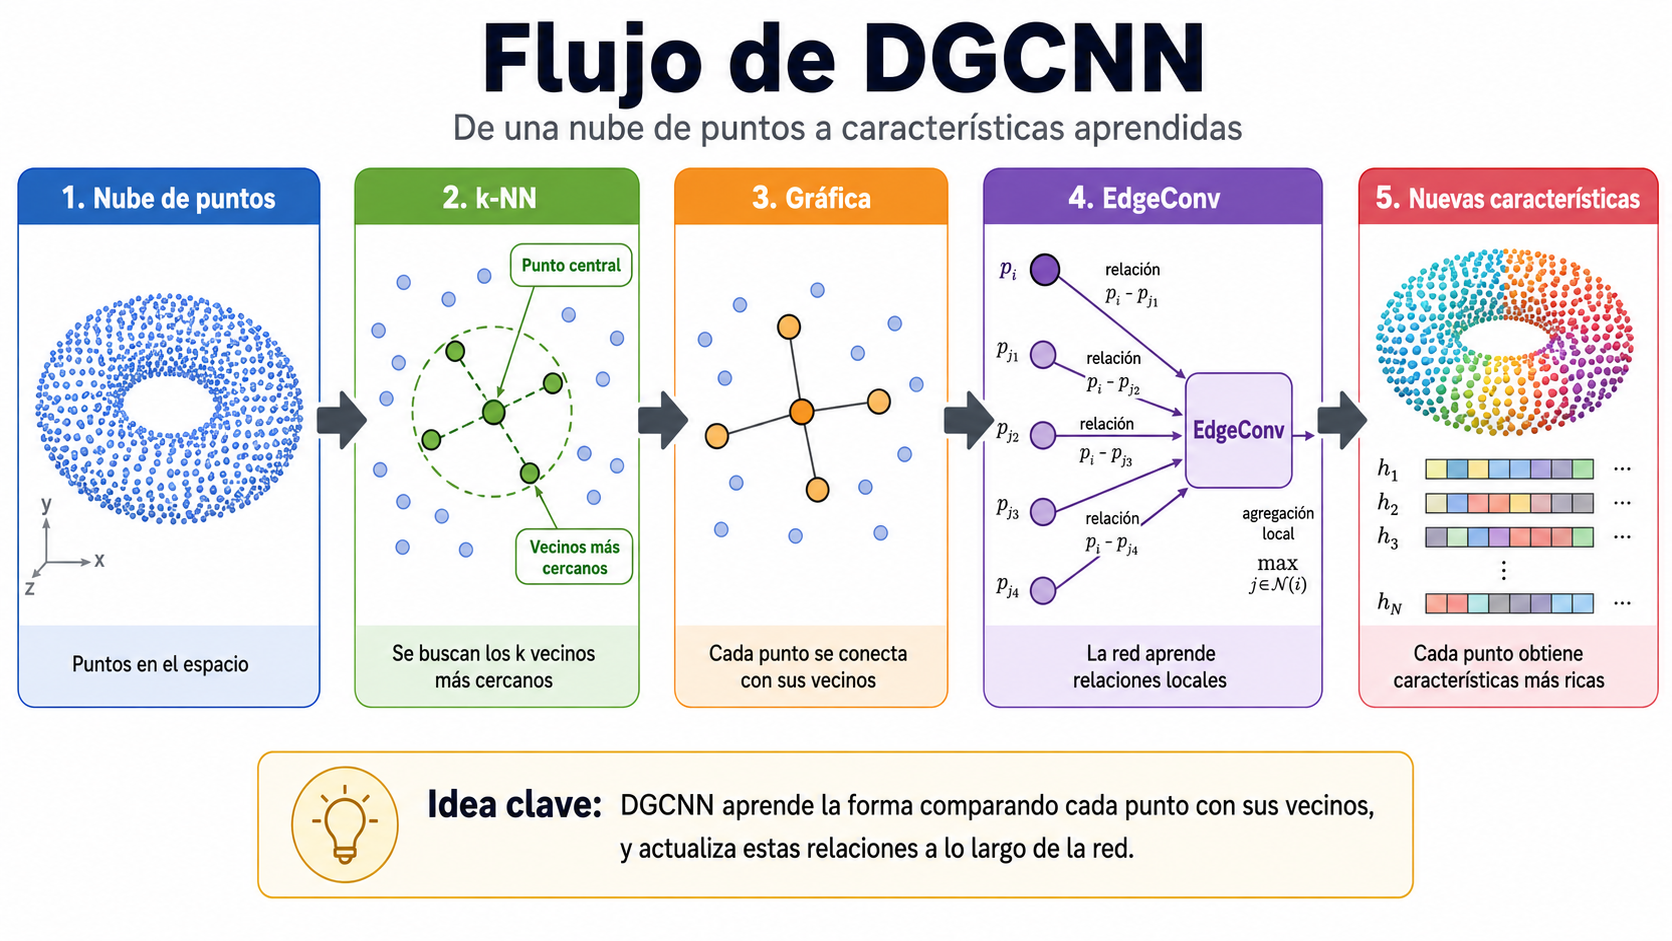
\includegraphics[width=\textwidth]{img/DGCNN.png}
    \caption{Flujo de la operación EdgeConv en DGCNN.}
    \label{fig:DGCNN}
\end{figure}


La operación central de DGCNN es EdgeConv, definida como

\[\max_{j \in \mathcal{N}k(i)}
\phi\theta
\left(
h_i^{(l)},
h_j^{(l)} - h_i^{(l)}
\right),
\]

donde $(h_i^{(l)})$ representa la característica del punto $(i)$ en la capa $(l)$, $(\mathcal{N}k(i))$ es el conjunto de sus $(k)$ vecinos más cercanos, $(\phi\theta)$ es una función aprendible, usualmente implementada mediante una red MLP, y la operación $(\max)$ agrega la información de los vecinos.

\subsection{PointNet}

PointNet es una arquitectura diseñada para procesar directamente nubes de puntos. Cada punto contiene normalmente coordenadas trdimensionales $(x,y,z)$, por lo que no es necesario transformar previamente el objeto en imágenes o vóxeles.Su principal propiedad es la invariancia ante permutaciones, es decir, el resultado no depende del orden en que se presenten los puntos de entrada, por lo que PointNet está diseñada para producir el mismo resultado aunque los puntos se presenten en un orden diferente. Esto se logra mediante el uso de operaciones simétricas, como la función $(\max)$, que agregan información de todos los puntos sin importar su orden.Así, PointNet puede obtener una representación global de la forma que puede utilizarse para tareas de clasificación o segmentación.

\begin{figure}[H]
    \centering

    % Primera imagen
    \begin{subfigure}[t]{0.85\textwidth}
        \centering
        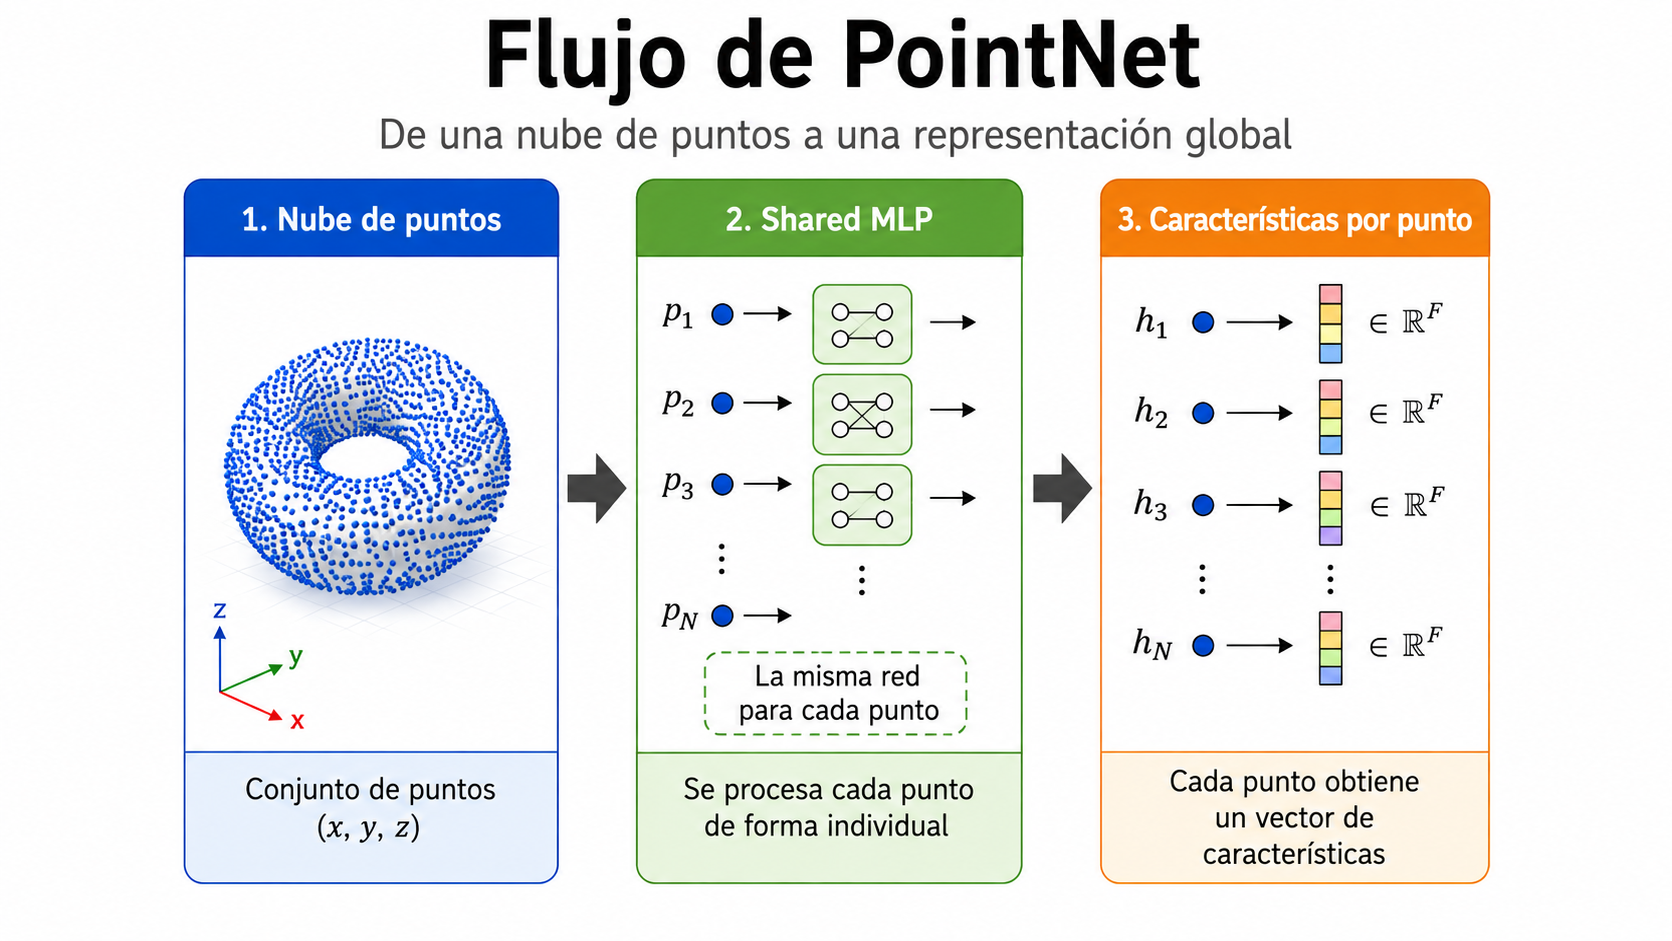
\includegraphics[width=\textwidth]{img/pointnet1.png}
        \label{fig:pointnet1}
    \end{subfigure}
    \vspace{0.1cm}
    % Segunda imagen
    \begin{subfigure}[t]{0.85\textwidth}
        \centering
        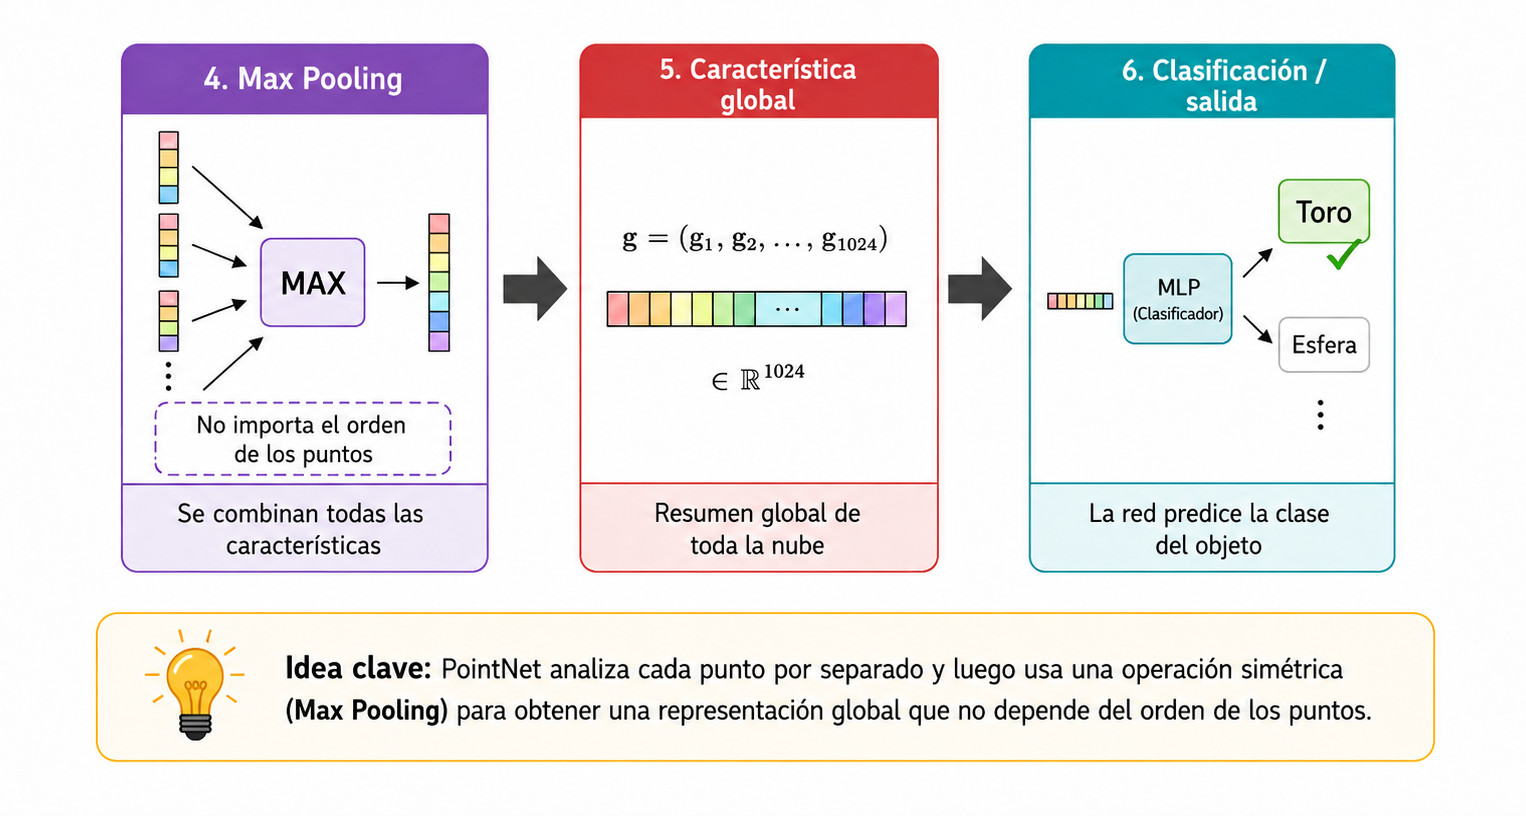
\includegraphics[width=\textwidth]{img/pointnet2.png}
        \label{fig:pointnet2}
    \end{subfigure}

    \caption{Flujo de la arquitectura PointNet. La primera imagen muestra la transformación de cada punto mediante una red MLP, mientras que la segunda ilustra la agregación de características mediante la operación simétrica $\max$ y la posterior clasificación mediante otra red MLP.}
    \label{fig:flujo_pointnet}
\end{figure}
Dada una nube de puntos

\[
X = {x_1, x_2, \dots, x_n},
\qquad x_i \in \mathbb{R}^3,
\]

PointNet aproxima una función sobre conjuntos mediante

\[
f(X)
\approx
\gamma
\left(
\max_{i=1,\dots,n}
\phi(x_i)
\right),
\]

donde $(\phi)$ transforma cada punto de manera independiente, $(\max)$ es una operación simétrica que garantiza invariancia al orden, y $(\gamma)$ es una red que produce la representación global para la clasificación.

\subsection{PointNet++}

PointNet++ extiende PointNet incorporando una estructura jerárquica de agrupamiento local. En lugar de procesar todos los puntos de manera completamente independiente, PointNet++ selecciona algunos puntos representativos y construye al rededor de ellos vecindades locales.Cada uno de estas vecindades representa una pequeña región de la superficie y es procesado mediante una versión local de PontNet para extraer características de esa zona. Después, estas regiones pueden volver a agruparse para formar regiones más grandes, así , PointNet++ aprende características de la superficie a diferentes escalas, lo que permite capturar tanto información local como global.

\begin{figure}[H]
    \centering
    % Primera imagen
    \begin{subfigure}[t]{0.85\textwidth}
        \centering
        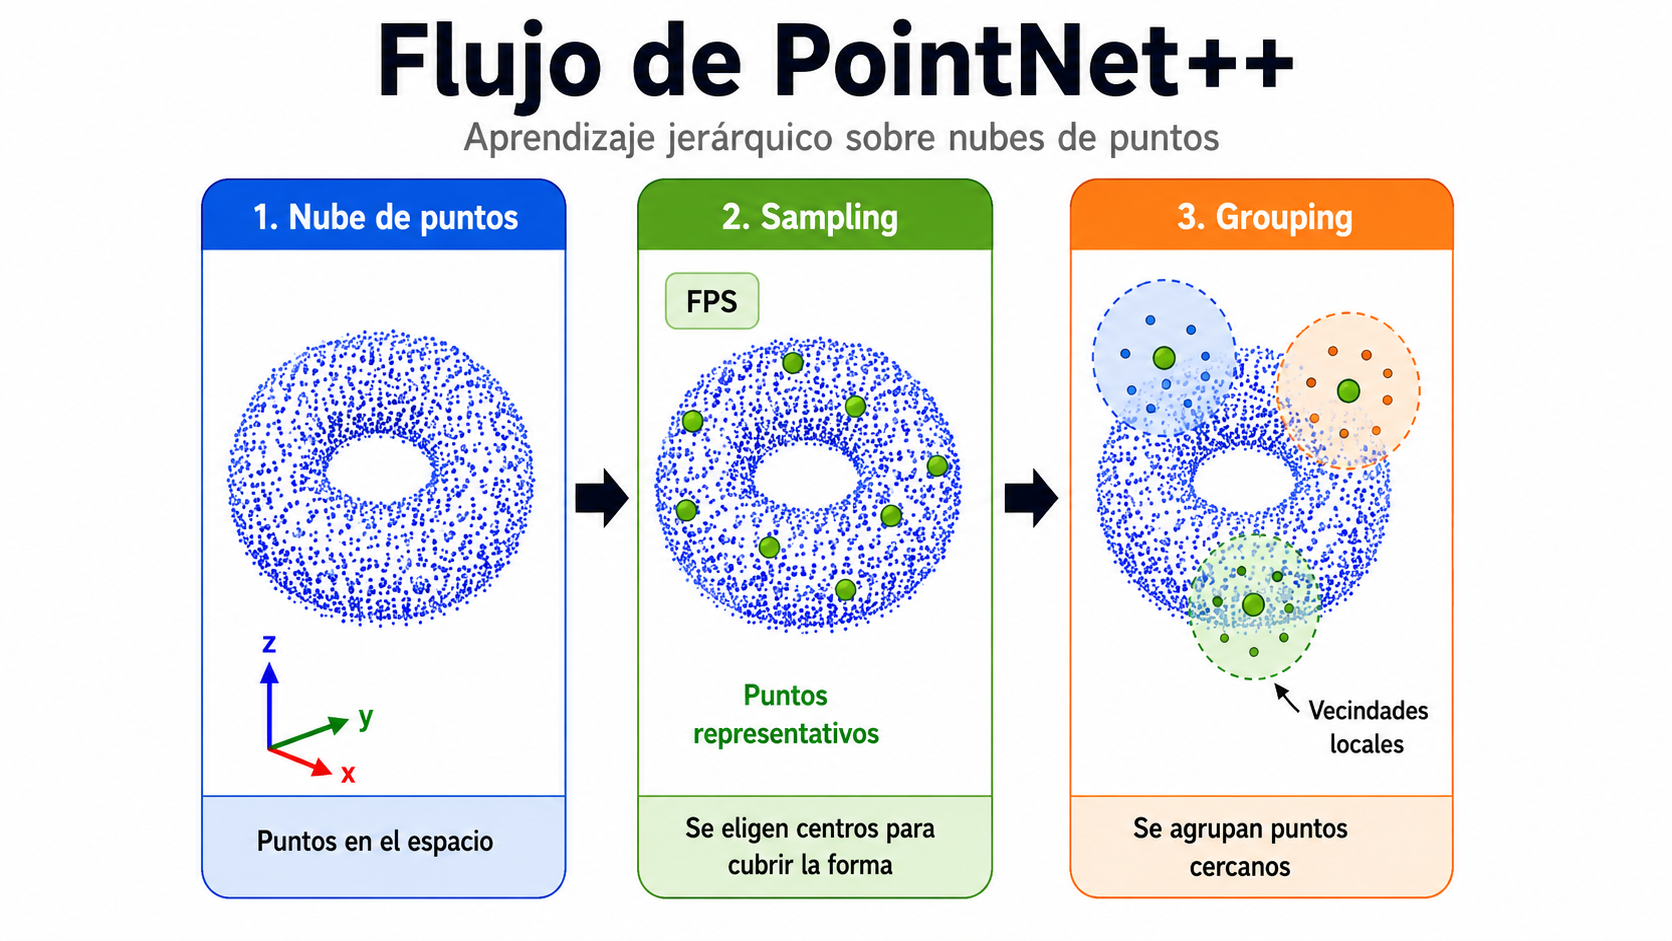
\includegraphics[width=\textwidth]{img/pointnetplus1.png}
        \label{fig:pointnetplus1}
    \end{subfigure}
    \vspace{0.1cm}
    % Segunda imagen
    \begin{subfigure}[t]{0.85\textwidth}
        \centering
        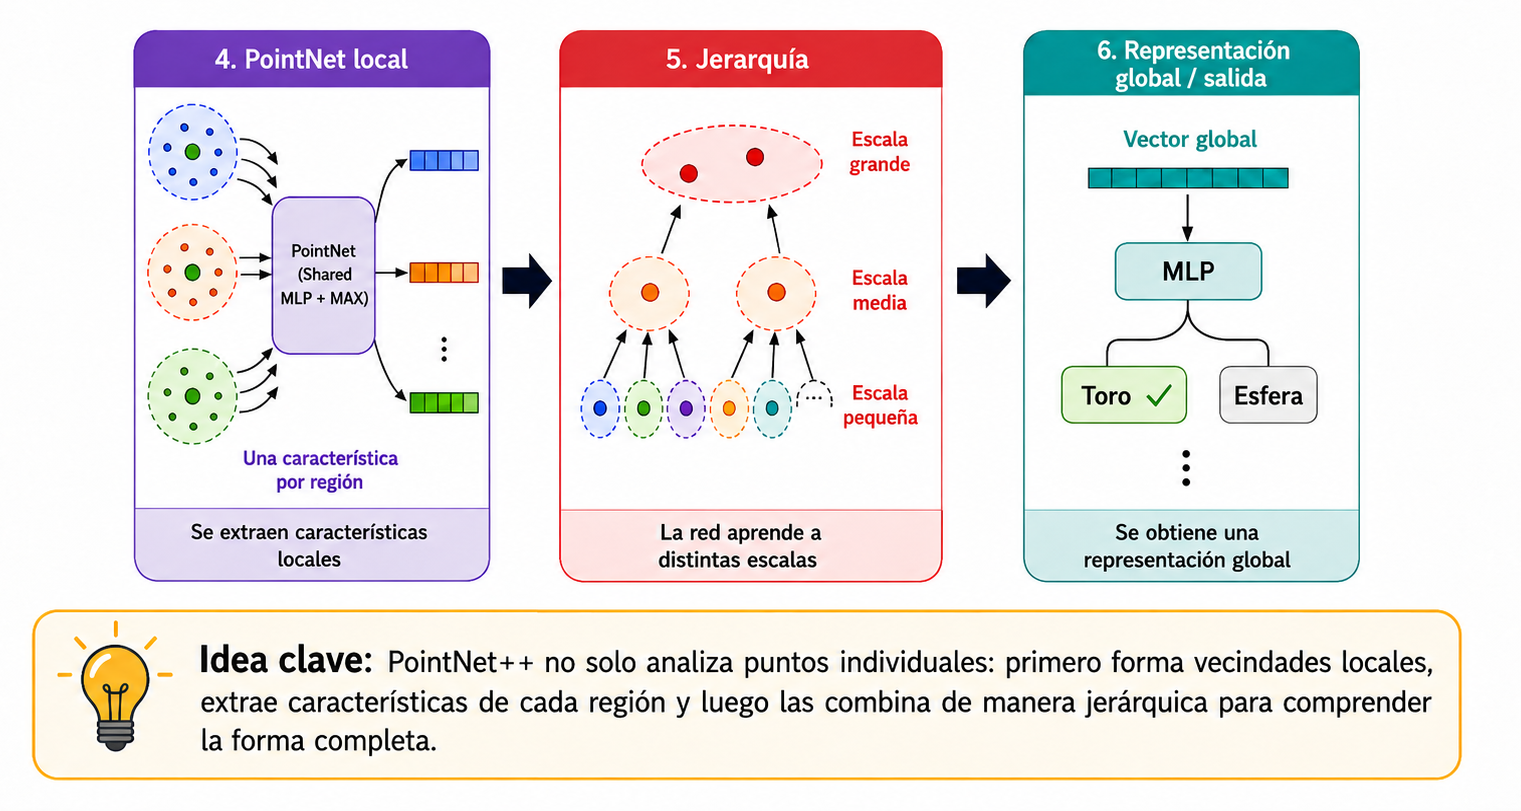
\includegraphics[width=\textwidth]{img/pointnetplus2.png}
        \label{fig:pointnetplus2}
    \end{subfigure}

    \caption{Flujo de la arquitectura PointNet++.}
    \label{fig:flujo_pointnet_plus}
\end{figure}

De forma esquemática, para un punto central $(x_i)$, se considera una vecindad local
\[
{x_j \in X : |x_j - x_i| \leq r},
\]

o bien una vecindad definida por (k) vecinos más cercanos. La representación local puede expresarse como
\[
\gamma
\left(
\max_{x_j \in \mathcal{N}(x_i)}
\phi
\left(
x_j - x_i
\right)
\right),
\]

donde $(x_j - x_i)$ representa la posición relativa de los puntos vecinos respecto al centroide $(x_i)$. Posteriormente, estas representaciones locales se combinan jerárquicamente para obtener una representación global de la nube de puntos.

\section{Diferencias clave}
Una vez descrita cada arquitectura que se ha utilizado para la evaluación de las superficies disponibles en la base de datos Eulearn, es importante destacar las diferencias clave entre ellas y a partir de estas diferencias, notar la importancia de la incorporación de información de adyacencias disponibles en las nuevas arquitecturas propuestas en \cite{2025eulearn}, así cómo la relevancia de los métodos de optimización propuestos en esta tesis.



\section{Análisis de resultados}

Con el objetivo de evaluar la efectividad del método de optimización propuesto en esta tesis, se realizaron diversos experimentos sobre el conjunto de datos EuLearn, el cual contiene superficies tridimensionales con distintas características topológicas. Se comparó el desempeño de diferentes arquitecturas de aprendizaje profundo utilizando las métricas de Precisión (Precision), Exhaustividad (Recall), Medida $F_{1}$ y Exactitud (Accuracy).

La Tabla \ref{tab:resultados_optimizacion} presenta los resultados obtenidos. En particular, se comparan arquitecturas tradicionales basadas en atención, operadores neuronales y procesamiento de nubes de puntos, contra las versiones optimizadas mediante el procedimiento desarrollado en este trabajo.

\begin{table}[H]
\centering
\caption{Comparación de resultados obtenidos con distintos modelos. Las variantes GS corresponden a arquitecturas que incorporan el método de optimización y preservación estructural propuesto en esta tesis.}
\label{tab:resultados_optimizacion}
\begin{tabular}{lcccc}
\toprule
\textbf{Modelo} & \textbf{Precisión} & \textbf{Recall} & \textbf{$F_{1}$} & \textbf{Accuracy} \\
\midrule
Attention (clásico) & 0.01 & 0.10 & 0.02 & 0.10 \\
FNO & 0.02 & 0.11 & 0.04 & 0.20 \\
DGCNN & 0.07 & 0.14 & 0.07 & 0.16 \\
PointNet (clásico) & 0.50 & 0.49 & 0.43 & 0.49 \\
PointNet++ & 0.50 & 0.54 & 0.52 & 0.63 \\
GS PointNet (propuesto) & 0.82 & 0.79 & 0.78 & 0.79 \\
GS Attention (propuesto) & 0.81 & 0.81 & 0.79 & 0.81 \\
\bottomrule
\end{tabular}
\end{table}

Los resultados muestran que las arquitecturas tradicionales presentan dificultades para capturar propiedades topológicas globales de las superficies. Esto se observa particularmente en los modelos basados en atención y en DGCNN, cuyos valores de precisión y exactitud permanecen por debajo del $20\%$.

Por otra parte, las arquitecturas diseñadas específicamente para el procesamiento de nubes de puntos, como PointNet y PointNet++, muestran una mejora considerable, alcanzando exactitudes de $49\%$ y $63\%$, respectivamente. Estos resultados sugieren que la incorporación de información geométrica local permite una mejor representación de las superficies, aunque todavía existen limitaciones para capturar adecuadamente características topológicas globales.

La principal contribución de este trabajo se refleja en las variantes GS PointNet y GS Attention, las cuales incorporan el método de optimización desarrollado en esta tesis. Dicho procedimiento realiza una reducción estructurada de la representación original preservando relaciones de adyacencia y propiedades topológicas relevantes. Como consecuencia, ambas arquitecturas obtienen los mejores resultados experimentales.

En particular, GS Attention alcanzó una exactitud del $81\%$ y una medida $F_{1}$ de $0.79$, mientras que GS PointNet obtuvo una precisión de $0.82$ y una exactitud del $79\%$. Estos valores representan mejoras significativas respecto a sus contrapartes tradicionales.

Comparando directamente PointNet++ con GS Attention, se observa un incremento absoluto de $18$ puntos porcentuales en exactitud ($63\%$ frente a $81\%$), lo que equivale a una mejora relativa aproximada del $28.6\%$. Asimismo, la medida $F_{1}$ aumenta de $0.52$ a $0.79$, evidenciando una mejor capacidad para identificar correctamente las distintas clases topológicas presentes en el conjunto de datos.

Estos resultados permiten concluir que el método de optimización propuesto contribuye de manera significativa a la preservación de información estructural relevante para el aprendizaje. La mejora observada en todas las métricas evaluadas sugiere que la estrategia desarrollada facilita la extracción de características topológicas discriminativas, permitiendo a las redes neuronales capturar propiedades globales de las superficies con mayor efectividad.

\section{Conclusiones}